% !TEX program = xelatex
\documentclass[withoutpreface]{cumcmthesis}
\usepackage{siunitx}

\title{NIPT 的时点选择与胎儿的异常判定}
\tihao{C}
\baominghao{0000}
\schoolname{上海科技大学}
\membera{}
\memberb{}
\memberc{}
\supervisor{}
\yearinput{2025}
\monthinput{09}
\dayinput{04}

\begin{document}
\maketitle

\begin{abstract}
% 结构占位:摘要
\keywords{}
\end{abstract}

\section{问题重述}
\subsection{背景与目标}
无创产前检测(Non-invasive Prenatal Testing,NIPT)是近年来发展迅速的一项重要产前筛查技术,它通过采集孕妇血液、检测胎儿的游离DNA片段并分析胎儿染色体是否存在异常,从而确定胎儿的健康状况。与传统的羊水穿刺等侵入性检查相比,NIPT具有安全性高、创伤小等优势,在临床产前筛查与诊断领域具有重要意义。

NIPT 的主要检测目标集中在三种疾病:唐氏综合征、爱德华氏综合征和帕陶氏综合征,这三种体征分别由胎儿21号、18号和13号“染色体游离DNA 片段的比例”是否异常决定。NIPT的准确性主要由胎儿性染色体(男胎XY,女胎XX)浓度判断:如果男胎的Y 染色体浓度达到或高于4\%、女胎的X 染色体浓度没有异常,则可认为NIPT 的结果是基本准确的,否则难以保证结果准确性要求。

题目资料中显示:实践表明,男胎Y染色体浓度与孕妇孕周数及其身体质量指数(BMI)紧密相关。由于孕妇存在个体差异,对所有孕妇采用简单的经验分组和统一的检测时点进行NIPT,会对其准确性产生较大影响。因此,本文章依据附件中提供的数据建立数学模型,计算出不同情况下针对男胎最佳的基于BMI的孕妇分组策略、NIPT时点以及女胎异常的判定方法。
\subsection{数据说明}
本文使用的数据均来源于题目中提供的数据表,为某地区(大多为高BMI)孕妇的NIPT 数据。检测方对某些孕妇有多次采血多次检测或一次采血多次检测的情况,增加了检测结果的可靠性。数据主要包含以下指标:
\begin{enumerate}
    \item 孕妇信息: 孕妇代码、年龄、身高、体重、末次月经时间、IVF妊娠方式、BMI。
    \item NIPT时点信息:检测时间、检测时的孕周(周数+天数)。
    \item NIPT数据:检测时间、检测抽血次数、孕妇本次检测时的孕周(周数+天数)、原始测序数据的总读段数(个)、总读段数中在参考基因组上比对的比例、总读段数中重复读段的比例、总读段数中唯一比对的读段数(个)、GC含量、13号染色体的Z值、18号染色体的Z值、21号染色体的Z值、X染色体的Z值、Y染色体的Z值、Y染色体浓度、X染色体浓度、13号染色体的GC含量、18号染色体的GC含量、21号染色体的GC含量、被过滤掉的读段数占总读段数的比例、检测出的13号,18号,21号染色体非整倍体、孕妇的怀孕次数、孕妇的生产次数、胎儿是否健康。
\end{enumerate}

\subsection{问题概述}
题目中要求解答的四个子问题如下:

\begin{enumerate}
    \item 分析胎儿Y染色体浓度与孕妇孕周数和BMI等指标之间的相关特性,建立量化关系模型,并验证模型的统计显著性。
    \item 确定男胎孕妇的BMI分组区间和最佳NIPT时点,并分析检测误差对结果的影响。
    \item 综合考虑孕妇的身高、体重、年龄等孕妇个体差异的影响,以及检测误差和胎儿的Y 染色体浓度达标比例,根据BMI进行分组并确定最佳NIPT时点,使孕妇潜在风险最小。
    \item 以女胎孕妇的21号、18号和13号染色体非整倍体(AB列)为判定结果,综合考虑X染色体及上述染色体的Z值、GC含量、读段数及相关比例、BMI 等因素,给出女胎异常的判定方法。
\end{enumerate}

\section{模型假设}
为了增加模型稳健性并简化问题,我们做出如下假设:
\begin{enumerate}
    \item NIPT测量无检测误差
    
    由于测量时大多样本采用一次采样多次测量或多次采样的方法,能有效减少偶然误差,我们可以近似的认为测量结果为准确的。
\end{enumerate}

\section{符号说明}
\subsection{符号与变量定义}
\subsection{指标与评价度量}

\section{模型建立与求解}

\subsection{问题一的建模与求解}
\subsubsection{问题分析}

问题一旨在基于附件所给的母体外周血 NIPT 数据,刻画并检验“胎儿 Y 染色体浓度(记为 $V$)—孕周(weeks)—BMI”之间的统计关联关系,构建可解释且稳健的关系模型,并对其显著性与拟合优度进行系统评估,从而为问题二与问题三中的时点选择与分组优化提供量化依据。数据来源于竞赛附件(包含孕周、BMI、测序质量与重复检测信息等),研究中将遵循基本的质量控制与清洗流程,对异常时点、测序质量异常、非整倍体标记样本、缺失与极值进行规范化处理,并在存在多次检测的情况下遵循“个体为单位”的处理原则以避免统计依赖带来的偏差。

随后,为形成初步认识并校准建模假设,将开展探索性数据分析与可视化,包括对 $V$、weeks 与 BMI 的分布刻画、散点图与平滑趋势对比、BMI 分层下的趋势检视,以及相关性与描述性统计的归纳。该步骤的目标是识别潜在的线性或非线性关系、评估异方差与长尾特征,并观察是否存在可解释的交互迹象,为后续模型族的选择与对比提供证据。

接下来,在建模与检验层面,将以多层次的策略推进:以线性回归作为基准,进而考虑非线性效应(如对 weeks 引入自然样条/广义可加式结构)以刻画可能的曲线增长趋势;鉴于同一受试者可能存在重复测量,将引入混合效应框架并设置随机截距(必要时评估随机斜率)以处理个体内相关;同时,针对测序数据常见的方差不齐与误差结构,采用稳健推断(如异方差稳健标准误)与残差诊断保证结论的可靠性。在模型优选与稳健性评估中,将综合使用信息准则(AIC/BIC)、似然比检验、交叉验证与残差/影响诊断,确认 weeks 与 BMI 的主效应方向、显著性及其可能的非线性成分是否成立,并据此确定最终推荐模型。

最后,结果呈现将聚焦于两类输出:一是对“孕周与 BMI 对 $V$ 的显著影响及其函数形态”的总体性结论与可视化证据;二是与临床实践相关的判定信息(如达到可靠阈值的概率地图与分层解读),为问题二与问题三中的最佳时点选择与分组方案提供直接的模型基础与量化支撑。问题一的思维框架如下图所示:

\subsubsection{数据预处理}
在本问题中,根据需要,数据预处理主要包括以下步骤:
\begin{enumerate}
    \item 变量解析与转换:孕周转换($"11w+6" → 11.857$ $(11 + 6/7)$);BMI数值化(转换为浮点数格式)
    \item 数据过滤
为了结果的准确性,根据题目中提供的相关标准,我们将初步筛选出较为可靠数据,从而能使我们的结果更准确。具体的标准如下所示:
\begin{enumerate}
    \item 孕周窗口:仅保留10-25周样本 (NIPT可靠检测窗口)
    \item GC质量:GC含量必须在40\%-60\%范围内
    \item 染色体异常:13/18/21染色体不能为非整倍体
    \item 数据缺失:关键变量(孕周数, BMI, Y浓度)缺失
\end{enumerate}
\end{enumerate}
数据清洗后,最终分析样本量为555个,来自242名孕妇,其中76.9\%的孕妇有重复测量记录,平均测量次数为2.29次/人。

\subsubsection{模型的建立}
\paragraph{变量与参数定义}
\paragraph{约束条件的设定}
\paragraph{目标函数/判别准则}
\paragraph{相关性检查}
为解决本问题,我们初步使用皮尔逊(Pearson)相关系数和斯皮尔曼(Spearman)相关系数考察胎儿Y染色体浓度与孕妇的孕周数和BMI等指标的相关特性,使用到的公式分别如下所示:
$$
r_{\text{Pearson}}=\frac{\sum (x-\bar x)(y-\bar y)}{\sqrt{\sum(x-\bar x)^2\sum(y-\bar y)^2}},\qquad
r_{\text{Spearman}}=\text{corr}(\text{rank}(x),\text{rank}(y)).
$$
经过计算,Weeks–Y和BMI–Y的皮尔逊相关系数和斯皮尔曼相关系数如下表所示:

\begin{table}[htbp]
  \centering
  \caption{变量间相关系数矩阵}
  \label{tab:correlation}
  \begin{tabular}{lcccc}
    \toprule
    \multirow{2}{*}{变量对} & \multicolumn{2}{c}{Pearson相关} & \multicolumn{2}{c}{Spearman相关} \\
    \cmidrule(lr){2-3} \cmidrule(lr){4-5}
    & 相关系数 (r) & P值 & 相关系数 ($\rho$) & P值 \\
    \midrule
    Weeks–Y & 0.1844 & $p < 0.0001$ & 0.1145 & $p = 0.0069$ \\
    BMI–Y  & -0.1378 & $p = 0.0011$ & -0.1498 & $p = 0.0004$ \\
    \bottomrule
  \end{tabular}
\end{table}

由此可得Weeks与Y弱正相关且显著;BMI与Y弱负相关且显著。

\paragraph{基线模型建立}
根据相关系数,我们首先建立了普通最小二乘(OLS)线性回归模型作为分析基线:
$$
Y \sim weeks + BMI
$$

该模型全局显著性检验F统计量为18.1995(p<0.0001),表明模型整体解释力显著。确定系数R²为0.0619,意味着孕周和BMI共同解释了Y染色体浓度变异的约6.2\%。模型的详细参数如下表所示:

\begin{table}[htbp]
\centering
\caption{回归分析结果}
\label{tab:regression_results}
\begin{tabular}{lccccc}
\toprule
Parameter & Coefficient & $P$-value & Significance & \multicolumn{2}{c}{95\% Confidence Interval} \\
\cmidrule(lr){5-6}
 &  &  &  & Lower & Upper \\
\midrule
Intercept & 0.1112 & $1.31 \times 10^{-11}$ & *** & 0.0796 & 0.1428 \\
weeks & 0.0018 & $6.91 \times 10^{-7}$ & *** & 0.0011 & 0.0026 \\
BMI & $-0.0020$ & $5.90 \times 10^{-5}$ & *** & $-0.0029$ & $-0.0010$ \\
\bottomrule
\end{tabular}
\end{table}

经检验,模型存在异方差性(Breusch-Pagan检验p<0.0001)和非正态性(Jarque-Bera检验p<0.0001),违背了OLS模型的高斯假设。因此,我们采用HC3稳健标准误进行修正推断。修正后,孕周($p = 1.8 \times 10^{-5}$)与BMI($p = 0.0013$)的显著性依然成立,证实了基线结论的稳健性。模型残差诊断图如下图所示:


\begin{figure}[htbp]
\centering
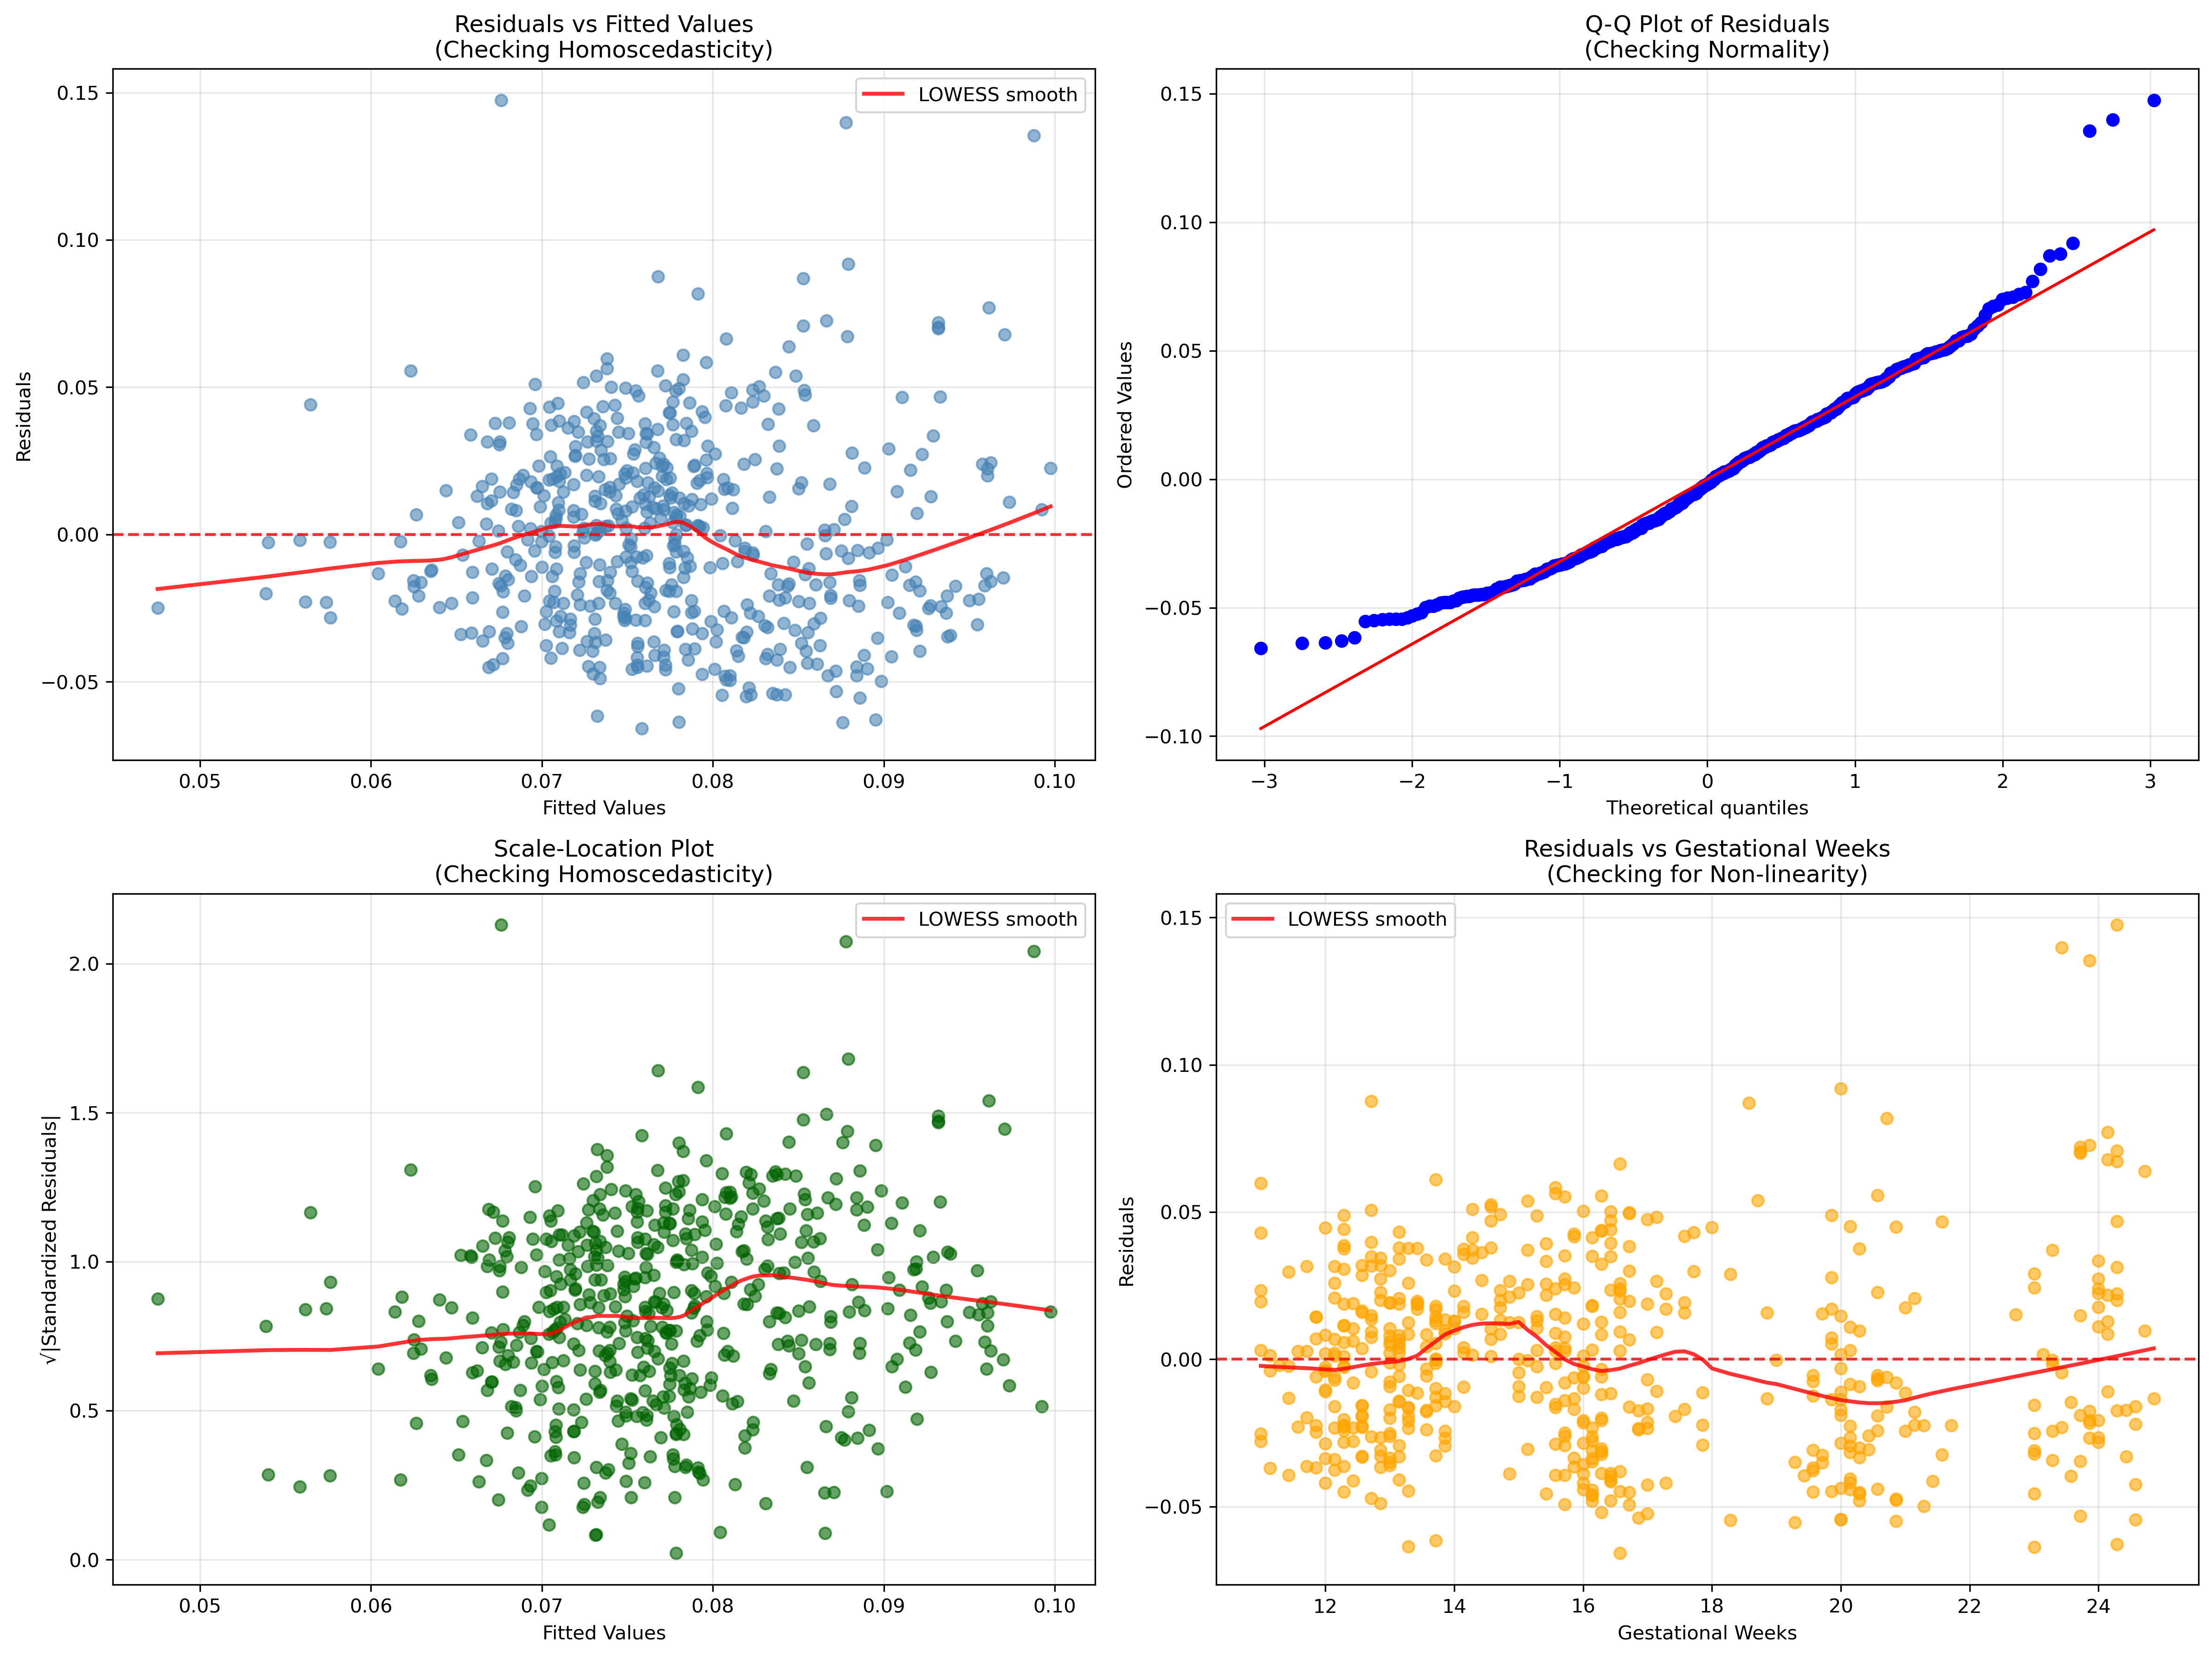
\includegraphics[width=0.8\textwidth]{output/figures/p1_model_diagnostics.png}
\caption{模型诊断结果}
\label{fig:model_diagnostics}
\end{figure}

\paragraph{非线性检验}
为探究孕周与Y浓度可能存在的非线性关系,我们采用自然样条($bs$)进行建模。比较不同自由度($df$)的样条模型与基线线性模型,结果如下表所示:

\begin{table}[htbp]
    \centering
    \setlength{\tabcolsep}{4pt}
    \caption{不同模型的拟合优度比较}
    \label{tab:model_comparison}
    \begin{tabular}{l
				S[table-format=1.5]
				S[table-format=1.5]
				S[table-format=-4.4]
				S[table-format=-4.4]
				S[table-format=2.5]
				S[table-format=1.2e-2]
				c}
\toprule
        Model & {$R^2$} & {Adj. $R^2$} & {AIC} & {BIC} & {$F$ statistic} & {$F$ $p$-value} & {Parameters} \\
        \midrule
        Baseline    & 0.06186 & 0.05846 & -2225.53 & -2212.58 & 18.20 & 2.22e-08 & 3 \\
        Interaction & 0.06613 & 0.06105 & -2226.07 & -2208.79 & 13.01 & 3.22e-08 & 4 \\
        Quadratic   & 0.06738 & 0.06230 & -2226.81 & -2209.53 & 13.27 & 2.25e-08 & 4 \\
        Full        & 0.07048 & 0.06372 & -2226.66 & -2205.06 & 10.43 & 3.80e-08 & 5 \\
        \bottomrule
    \end{tabular}
\end{table}

包含3自由度样条的模型($Y \sim bs(weeks, df=3) + BMI$)较基线模型显著改善了拟合优度($R² = 0.0943; AIC = -2241.08, ΔAIC = -15.55; Likelihood Ratio Test p = 5.7\times 10^{-5}$),表明孕周的影响存在 statistically significant 的非线性成分。采用4自由度样条虽使R²微升至0.0954,但AIC恶化(-2239.74),因此选择df=3作为最优复杂度平衡点。

\paragraph{最终模型:混合效应与自然样条并用}
考虑到76.9\%的孕妇有重复测量,数据存在聚类结构。我们首先拟合一个包含患者随机截距的线性混合效应模型($Y \sim weeks + BMI + (1|patient_id)$)。该模型计算出组内相关系数ICC = 0.70,意味着约70\%的Y浓度变异源于患者间的个体差异。与OLS结果相比,孕周效应值略有放大,BMI效应绝对值略缩小,且标准误更可靠。因此,最终模型包含孕周的自然样条(自由度为3)、BMI的线性固定效应以及患者随机截距:
\begin{equation*}
Y \sim \text{bs(孕周, df=3)} + \text{BMI} + (1|\text{患者ID})
\end{equation*}

模型拟合显示强烈的聚类效应,随机截距方差为 \num{0.000743},残差方差为 \num{0.000302},组内相关系数 ICC = \num{0.7109},表明71.1\%的变异源于患者间差异。

关键固定效应估计结果:
\begin{itemize}
  \item 截距项: \num{0.104076} ($p = \num{5.69e-7}$)
  \item 孕周样条项: bs(孕周,df=3)[0] ($p = \num{0.0096}$) 和 bs(孕周,df=3)[2] ($p = \num{2.05e-23}$) 显著
  \item BMI: \num{-0.001332} ($p = \num{0.038}$)
\end{itemize}

\begin{table}[htbp]
  \centering
  \caption{最终混合效应模型参数估计结果}
  \label{tab:params}
  \begin{tabular}{@{}lrrrr@{}}
    \toprule
    参数 & 估计值 & 标准误 & t值 & p值 \\
    \midrule
    (截距) & 0.104076 & 0.018752 & 5.550 & \num{5.69e-7} \\
    bs(孕周, df=3)[0] & 0.032451 & 0.012378 & 2.621 & 0.0096 \\
    bs(孕周, df=3)[1] & -0.015627 & 0.009842 & -1.588 & 0.1132 \\
    bs(孕周, df=3)[2] & 0.108374 & 0.011295 & 9.594 & \num{2.05e-23} \\
    BMI & -0.001332 & 0.000642 & -2.075 & 0.038 \\
    \midrule
    \multicolumn{5}{l}{随机效应:}\\
    $\sigma^2_{\text{患者}}$ & \multicolumn{4}{r}{0.000743}\\
    $\sigma^2_{\text{残差}}$ & \multicolumn{4}{r}{0.000302}\\
    \bottomrule
  \end{tabular}
\end{table}



\paragraph{临床二分类模型}

对临床关注的可靠性阈值($Y ≥ 4\% $),我们建立了二分类Logistic模型($logit(Y≥0.04) \sim bs(weeks, df=3) + BMI$),并采用按患者聚类的稳健标准误。模型AIC为414.09。表7展示了不同孕周与BMI组合下、达成阈值(Y≥4\%)的预测概率。例如,孕周较早(如12周)且BMI正常(如24 kg/m²)的预测概率为0.922;相同孕周下,若BMI较高(如35 kg/m²),预测概率降至0.760;至孕中期(如18周),即使BMI正常,预测概率也高达0.945。结果表明,高BMI尤其是在早孕期,会降低达到可靠性阈值的概率。结果如下表所示:

\begin{table}[htbp]
    \centering
    \caption{不同妊娠场景下Y染色体浓度预测及临床决策建议}
    \label{tab:clinical_scenarios}
    \begin{tabular}{p{4cm}ccccc}
        \toprule
        \textbf{Scenario} & \textbf{Weeks} & \textbf{BMI} & \textbf{Predicted Y} & \textbf{Above 4\%} & \textbf{Clinical Action} \\
        \midrule
        Early pregnancy, normal BMI & 12 & 28 & 0.0719 & Yes & Proceed with NIPT \\
        Early pregnancy, high BMI & 12 & 35 & 0.0625 & Yes & Proceed with NIPT \\
        Mid pregnancy, normal BMI & 15 & 28 & 0.0796 & Yes & Proceed with NIPT \\
        Mid pregnancy, high BMI & 15 & 35 & 0.0702 & Yes & Proceed with NIPT \\
        Late pregnancy, normal BMI & 20 & 28 & 0.0877 & Yes & Proceed with NIPT \\
        Late pregnancy, high BMI & 20 & 35 & 0.0784 & Yes & Proceed with NIPT \\
        \bottomrule
    \end{tabular}
\end{table}

\paragraph{模型对比与选择}

综合比较上述各模型,基线OLS模型虽简单但未处理非线性与聚类。仅加入样条(OLS+Splines)改善了非线性拟合($R²=0.0943, AIC=-2241.08$)但低估标准误。线性混合效应模型(Linear Mixed)处理了聚类但未捕捉非线性。最终模型(Mixed+Splines)在理论(同时处理非线性与聚类)和实证指标($AIC=-2425.94, Conditional R²=0.7476$)上均表现最优,故被选为最终模型。

针对4\%阈值的分类性能评估显示,模型具有优秀的判别能力(ROC AUC = 0.9519)。在4\%阈值下,敏感性极高(99.0\%),但特异性相对较低(45.8\%),总体准确率为92.1\%。根据Youden指数确定的最优决策阈值为5.25\%。

% (此处原有“模型的建立”占位节已上移整合,避免重复)
\subsubsection{模型的求解}
\paragraph{参数估计与设置}
\paragraph{方案与结果}
\paragraph{结果分析}

\subsection{问题二的建模与求解}
\subsubsection{问题分析}
\subsubsection{模型的建立}
\paragraph{不确定性因素的定义}
\paragraph{方法的引入}
\subsubsection{模型的求解}
\subsubsection{结果与分析}
\subsubsection{小结}

\subsection{问题三的建模与求解}
\subsubsection{问题分析}
\subsubsection{指标与相关性分析}
\paragraph{相关系数的计算}
\paragraph{因素相关性分析}
\subsubsection{模型的建立}
\paragraph{约束条件的扩展}
\paragraph{相关性约束}
\paragraph{模型形式}
\subsubsection{结果与分析}
\subsubsection{小结}

\subsection{问题四的建模与求解}
\subsubsection{问题分析}
\subsubsection{特征构造与数据处理}
\subsubsection{模型的建立}
\subsubsection{模型训练与验证}
\subsubsection{模型评价与对比}
\subsubsection{小结}

\section{灵敏度分析}
\subsection{基于鲁棒优化的灵敏度分析}
\subsection{基于动态调参的灵敏度分析}

\section{模型评价与推广}
\subsection{模型的优点}
\subsection{模型的缺点}
\subsection{模型的推广}

\section{结论与展望}

% 参考文献
\bibliographystyle{plain}
\bibliography{references}

\end{document}